\chapter{First-Order Differential Equations}

In this chapter, methods will be given for solving first- order differential equations. First-order means that the first derivative of the unknown function is the highest derivative appearing in the equation. This implied that the most general first-order differential equation has the form $F(t,x,t')=0$ for some function $F$, in this chapter, we will assume that the equation can be solved explicitly for $x'$. This means that our first-order differential equations can always be put in the form:

\begin{equation}
  x'=f(t,x)
\end{equation}

where $f$ denotes an arbitrary function of two variables. To see why such an assumption makes sense,supposed the differential equation is:

\begin{equation}
  (x'(x))^2+4x'(t)+3x(t)=t.
\end{equation}

It would be messy, but not impossible to use the quadratic formula to extract two differential equations of the form $x'=f(t,x)$ from this quadratic equation. However, one could also imagine equations where solving for $x'(t)$ is not even possible, and in such a case, some of our methods might not be applicable.

The material in this chapter will cover several analytic methods for solving first-order differential equations, each requiring the function $f$ to have a special form. Two different graphical methods are also described; one for the general equation depending only on $x$. Numerical methods for first-order equations are introduced and theoretical issues of existence and uniqueness of solutions are discussed.

\section{Separable First-Order Equations}

  The first analytic method we will consider applies to first-order equations that can be written in the form

  \begin{equation}
    \frac{dx}{dt} = g(t)h(t);
  \end{equation}

  that is, when the function $f(t, x)$ can be factored into a product of a function of $t$ times a function of $x$. Such a differential equation is called separable. 

  \begin{problem}
    Determine which of the following first-order differential equations are separable. Hint: try to factor the right- hand side if the equation does not initially appear to be separable.

    \begin{equation}
      x' = xt + 2x\to x' = x(t + 2)\to g(t) = t + 2,h(x) = x\\
    \end{equation}

    \begin{equation}
      x' = x + \cos (t)\\
    \end{equation}
    
    \begin{equation}
      x' = xt^2 + t^2 - tx\to x' =(t^2 - t)(x + 1)\to g(t) =(t^2 - t),h(x) =(x + 1)\\
    \end{equation}

    \begin{equation}
      x' = x^2 + x + 3\to x' = (1)(x^2 + x + 3)\to g(t) = 1,h(x) = x^2 + x + 3
    \end{equation}

    \begin{enumerate}
      \item 
        If $h(x) = 1,$ the separable equation $x'=g(t)$ is just an integrating problem and the solution is 
        \begin{equation}
          x=\int g(t)dt;
        \end{equation}
        that is, $x$ is just the **indefinite integral** of the function $g(t)$. Remember that this means that $x$ can be *any* function $G(t)$ such that $G'(t)=g(t)$, and this introduces an arbitrary constant into the solution. As an example, the solution of $x'=t+1$ is 

        \begin{equation}
          x(t)=\int(t+1)dt=\frac{t^2}{2}+t+ c
        \end{equation}

        Even in this simple case the solution is an infinite one-parameter family of functions.
      
      \item If $g(t)=1$, the separable equation $x'=h(x)$ is called an **autonomous** first-order differential equation. Unless $h(x)$ is a constant, it is no longer possible to solve the equation by simple integration, and the method given below must be used. Autonomous first-order differential equations are important and will be investigated more thoroughly in section 2.7. In the above examples, only the last equation is autonomous. The other three contain functions of $t$ (other than the unknown function $x(t)$) on the right-and side.
    \end{enumerate}
  \end{problem}

  \begin{problem}
    Solve the differential Equation $\frac{dx}{dt}=-tx^2$.

    Solution. Split $dx/dt$ into two pieces, $dx$ and $dt$, and do a bit of algebra to write:

    \begin{equation}
      - \frac{dx}{x^2} = tdt
    \end{equation}

    Integrate each side with respect to its own variable to obtain:

    \begin{equation}
      \int \left( - \frac{1}{x^2}\right) =\int tdt\to \frac{1}{x} = \frac{t^2}{x} + C.
    \end{equation}

    where the arbitrary constants on each side have been collected on the right. Solve this equation for x to obtain the one parameter family of solutions

    \begin{equation}
      x=\frac{1}{(t^2/2)+C}.
    \end{equation}

    We should check that the function $x(t)$ does satisfy the differential equation for any value of the constant C. It appears that this method works, but splitting $dx/dt$ into two pieces is not a mathematically condoned operation; therefore, a justification of the method needs to be given.

    If an equation is separable, and $x'(t)$ is written as $dx/dt$, both sides of the equation $dx/dt=g(t)h(x)$ can be divided by $h(x)$, and the equation becomes

    \begin{equation}
      \frac{1}{h(x(t))}\left(\frac{dx}{dt}\right)dt=\int g(t)dt+C.
    \end{equation}

    The method of simple substitution can be applied to the integral on the left. If we substitute $u=x(t)$, then $du=(dx/dt)dt$, and the equation becomes

    \begin{equation}
      \int\frac{1}{h(u)}du=\int g(t)dt+C.
    \end{equation}

    Now let $H(u)$ be any function such that $H'(u)=1/h(u)$ and $G(t)$ any function with $G'9t)=g(t)$. Then the equation above implies that

    \begin{equation}
      H(u)+C_1=G(t)+C_2\to H(u)=G(t)+C,
    \end{equation}

    Where C is the constant $C_2-C_1$

    Replacing $u$ again by $x(t)$:

    \begin{equation}
      H(x(t))=G(t)+ C
    \end{equation}
  \end{problem}

  Check carefully that the expression $H(x)=G(t)+C$ is exactly the same as the solution obtained above. It is an **implicit solution** of $-dx/x^2=tdt$; that is, it defines a relationship between the unknown function $x$ and its independent variable $t$. If it can be solved explicitly for $x$ as a function of $t$, the result is called an **explicit solution of the differential equation. As expected, the integration produces an infinite on-parameter family of solutions

  \begin{theorem}
    TTo solve a separable first-order differential equation, $x'(t)=g(t)h(x)$:
    \begin{itemize}
      \item Write the equation in the form $dx/dt=g(t)h(x)$.
      \item Multiply both sides by $dt$, divide by $h(x)$, and integrate, to put the equation in the form 
        \begin{equation}
          \int \frac{1}{h(x)}dx =\int g(t)dt.
        \end{equation}
      \item Find any function $H(x)$ such that $H'(x)=1/h(x)$ and any function $G(t)$ such that %G'(t)=g(t).
      \item Write the solution as $H(x)=G(t)+C$
      \item If possible, solve the equation from the previous step explicitly for x, as a function of t.
    \end{itemize}
  \end{theorem}

\section{}
\section{}

\section{Existence and Uniqueness of Initial Value Problems}

  Given an initial value problem, how can I know that a solution exists, and if so, the uniqueness of that solution.

  \begin{problem}
    $\frac{dx}{dt}=\sqrt{x}$, $x(0)=0$ has two solutions. These solutions are $x(t)=\frac{t^2}{4}$ and $0$. We can change the initial condition to be $x(0)=5$. we can separate our values to get:

    \begin{equation}
      x(t) =\left(\frac{t}{2} + \sqrt{5}\right)^2
    \end{equation}
    
    If we change the initial condition to $x(5)=-5$ we get no solutions. We can also change the initial condition to $x(5)=0$ which gives us two solutions:

    \begin{align}
      x(t) =\left(\frac{t - 5}{2}\right)^2\\
      x(t) = 0
    \end{align}
  \end{problem}

\section{Exact Ordinary Differential Equations}

  This highlights an analytic technique to find the solutions to an ordinary differential equation. This technique depends on if we are able to write an ODE in the form $\frac{d}{dx}(F(x,y(x)))=0$. How can we tell if this is possible? 

    We can determine this by using the multi-variable chain rule from calculus 3:

    \begin{equation}
      \frac{d}{dx}(F(x,y(x))) = \frac{\partial F}{\partial x} + \frac{\partial F}{\partial y} \frac{dy}{dx} = 0 
    \end{equation}

    Now in order to actually solve the ordinary differential equation, we will turn the equation above into something that we can work with:

    \begin{equation}
      M(x,y) + N(x,y)\frac{dy}{dx} = 0
    \end{equation}

    Now we ask the question, does $f(x,y)$ exist such that $\frac{\partial F}{\partial x} =  M(x,y)$ and $\frac{\partial F}{\partial y} = N(x,y)$? We can test this by checking to see if we can do the following:

    \begin{equation}
      \frac{\partial^2F}{\partial x\partial y}=\frac{\partial^2 F}{\partial y\partial x}\rightarrow\boxed{\frac{\partial M}{\partial y}=\frac{\partial N}{\partial x}}
    \end{equation}

    If it passed the test, we use the equations to find $F(x,y)$, and then we can use $F(x,y(x))=C$ to find the solution to the problem.

    \begin{problem}
      Calculus 3 example. Consider a field $\vec{v}=<2y+4x,2x-5y>$. Is this a gradient field? If so, what is its potential function. In order to find this, there must be a function $f(x,y)$ such that $\bigtriangledown f=\vec{v}$.
    
    
      \begin{equation}
        {\partial f}{\partial y}\big>=<6xy,2x-5y>\\
      \end{equation}
  
      \begin{align}
        \frac{\partial f}{\partial x}=6xy,&& \frac{\partial f}{\partial y}=2x-5y
      \end{align}
  
      Therefore, we know that $f_{xy}=f_{yx}$ Now we just need to set the two equations equal to each other and solve:
  
      \begin{equation}
        \frac{\partial}{\partial y}(2y+4x)\stackrel{?}{=}\frac{\partial}{\partial x}(2x-5y)
      \end{equation}
  
      And we can solve that equation algebraicly and get $2=2$, therefore this is the solution to the ordinary differential equation
  
    \end{problem}

    \begin{problem}
      Solve $(4x+2y)+(2x-5y)\frac{dy}{dx}=0$. We should set $M(x,y)=4x+2y$ and set $N(x,y)=(2x-5y)$.

    \begin{enumerate}
      \item Testing to see if $\frac{\partial M}{\partial y}=\frac{\partial N}{\partial x}$
        \begin{equation}
          \frac{\partial}{\partial y}(4x+2y)\stackrel{?}{=}\frac{\partial}{\partial x}(2x-5y)
        \end{equation}
      \item Now we need to find $F(x,y)$:
        \begin{align}
          \frac{\partial F}{\partial x}=4x+2y && \frac{\partial F}{\partial y}=2x-5y\\
          F(x,y)=\int(4x+2y)dx=2x^2+2xy+c_y, && F(x,y)=\int(2x-5y)dy=2xy-\frac{5}{2}y^2+c_x
        \end{align}
        We can determine that $c_y=\frac{5}{2}y^2$ and $c_x=2x^2$ by looking at the two equations next to each other. Therefore, we know that $F(x,y)=2x^2+2xy-\frac{5}{2}y^2$.
    \end{enumerate}
    Our resulting solution is:

    \begin{equation}
      \boxed{2xy-\frac{5}{2}y^2+2x^2=C}
    \end{equation}

    This was an implicitly defined solution, so $F(x,y)=2xy-\frac{5}{2}y^2+2x$, and our ode is:
    
    \begin{align}
      \frac{d}{dx}\left[2xy(y)-\frac{5}{2}(y(x))^2+2x^2\right]=\frac{d}{dx}[C]\\
      (2y+2xy')-\frac{5}{2}2(y)+4x=0\\
    \end{align}

    \paragraph{Example 2} Solve the differential equation,
    
    \begin{equation}
      2x^2y+e^y+(x^3+xe^y-2y)\frac{dy}{dx}=0. 
    \end{equation}

    We can see that $3x^2y+e^y = M(x,y)$ and $(x^3+xe^y-2y)\frac{dy}{dx}=0$.

    We can test this by checking to see if:
    
    \begin{equation}
      \frac{\partial M}{\partial y}\stackrel{?}{=}\frac{\partial N}{\partial x}
    \end{equation}

    and by taking the partial derivatives of each of the equations, we can see that $3x^2+e^y=3x^2+e^y$. Now that we know that this is an exact ordinary differential equation, we need to solve for $F(x,y)$. In order to find $F(x,y)$, we must do 

    \begin{align}
      \frac{\partial F}{\partial x}=M && \frac{\partial F}{\partial y}=N.
      \end{align}

      This means that 

      \begin{align}
        F(x,y)=\int(3x^2y+e^y)dx && F(x,y)=\int(x^3+xe^y-2y)dy\\
        =x^3y+xe^y+C_y && =x^3y+xe^y-y^2+C_x\\
      \end{align}

      So, $F(x,y)=x^3yxe^y-y^2$, and our solution is:

      \begin{equation}
        \boxed{x^3y+xe^y-y^2=C}\\
      \end{equation}

      Now we need to find a solution that satisfies the initial value proble, $y(-2)=1$.
      
      \begin{align}
        (-2)^3(1)+(-2)e^1-(1)^2&=C\\
        -8-2e-1&=C\\
        -9-2e&=C\\
      \end{align}

      Which results in our particular solution being:

      \begin{equation}
        \boxed{x^3y+xe^y-y^2=-9-2e}
      \end{equation}
    \end{problem}

  \subsection{Substitution}
    Sometimes we can make a substitution that turns one ordinary differential equation into one that we can solve.
    
    \begin{problem}
      Let's take the equation $\frac{dy}{dx}=\frac{1-x-y}{x+y}$. In order to do this you need to trade out $y(x)$ for $u(x)$:

      \begin{equation}
        \frac{dy}{dx}=\frac{du}{dx}-1
      \end{equation}

      \begin{equation}
        \frac{du}{dx}-1=\frac{1-u}{u}=\frac{1}{u}-1
      \end{equation}

      After we do those steps, we can see that this is a separable ordinary differential equation, and we can use the normal method to solve a separable equation:

      \begin{equation}
        \begin{aligned}
          \int udu&=\int1dx\\
          \frac{u^2}{2}&=x+C\\
          u^2&=2x+D\leftarrow D=2C\\
          (x+y)^2&=2x+D\rightarrow x+y=\pm\sqrt{2x+D}\\
          y&=-x\pm\sqrt{2x+D}
        \end{aligned}
      \end{equation}

      Where the initial condition determines the last equation above. Now we need to solve for the initial condition of $y(6)=4$, and we can do this by just pluggin in the values, and determining the sign on the square root:

      \begin{equation}
        \begin{aligned}
           4&-6\pm\sqrt{12+D}\\
          10&=\pm\sqrt{12+D}\\
          D&=88\to y(x)=-x+\sqrt{2x+88}\\
        \end{aligned}
      \end{equation}
    \end{problem}

  \subsection{Bernoulli Ordinary Differential Equations}

    We use Bernoulli's solution to an ordinary differential equation if the equation can be written in the form $\frac{dx}{dt}+p(t)x=q(t)x^n$, where if $n=0$, the equation is linear and where if $n=1$, the equation is both linear and separable. We can do a substitution for Bernoulli ordinary differential equations where we let $v=x^{1-n}$, and we trade out $x(t)\to v(t)$ to turn the differential into a linear differential. Another formula we can use for pluggin in to find the separable ordinary differential equation is $\frac{du}{dx}+(1-n)p(x)u=(1-n)q(x)$, but we do not have an example to show for that method. 

    \begin{problem}
      Consider the Ordinary differential equation $t\frac{dy}{dt}+y=\frac{1}{y^2}$, and solve. Our first step for this problem is to divide both sides by $t$ to rearrange it into the Bernoulli form:

      \begin{equation}
        \frac{dy}{dt}+\frac{1}{t}y=\frac{1}{t}y^-2
      \end{equation}

      Because $y$ is our dependent variable, we will be looking for our $n$ value, and we will find it on the $y$ on the right hand side. This gives us $n=-2$. Now we need to let $v(t)=y^{1-(-2)}=y^3$ and this means that $y(t)=(v(t))^{1/3}$. Now wee need to take the differential of this equation in order to find a substitution for $\frac{dy}{dt}$:

      \begin{align}
        \frac{dy}{dt}=\frac{1}{3y^2}\frac{dv}{dt}\\
        \frac{dv}{dt}=3y^{-2}\frac{dy}{dt}\\
      \end{align}

      Once we have found a substitution for $\frac{dy}{dt}$, we can simply plug in our equation and solve for $v(t)$:

      \begin{equation}
        \frac{1}{3y^2}\frac{dv}{dt}+y=\frac{1}{y^2}
      \end{equation}

      \begin{equation}
        \frac{t}{3}\frac{dv}{dt}+y^3=1
      \end{equation}

      We solve for $v(t)$ and then we can use the integrating factors method to solve the ordinary differential equation:

      \begin{equation}
        \begin{aligned}
          \frac{dv}{dt}+\frac{3}{t}v&=\frac{3}{t}\\
          \mu(t)&=e^{\int\frac{3}{t}dt}=e^{3ln(t)}=t^3\\
          t^3\frac{dv}{dt}+3t^2v&=3t^2\\
          \frac{d}{dt}(t^3v)&=3t^2\\
          \int t^3v&=\int3t^2dt=t^3+C\\
          v(t)&=1+\frac{C}{t^3}\to y(t)=(v(t))^{\frac{1}{3}}\\
        \end{aligned} 
      \end{equation}\\

      Now we just need to let $v(t)=y^3$ and plug this back into the equation to get $y(t)=\left(1+\frac{C}{t^3}\right)^{\frac{1}{3}}$ as our final solution.
    \end{problem}

    Homogenius ordinary differential equations can be written in the form $\frac{dx}{dt}=f\left(\frac{x}{t}\right)$. This means that if we just substitute $v$ for $\frac{x}{t}$, we will turn the Homogenius equation into a separable ordinary differential equation.

    \begin{problem}
      Consider the homogenius ODE, $(5y-2x)\frac{dy}{dx}=4x+2y$. We can divide the $5y-2x$ so we will end up with the equation

      \begin{equation}
        \frac{dy}{dx}=\frac{4x+2y}{5y-2x}=\frac{4+\frac{2y}{x}}{5\frac{y}{x}-2}
      \end{equation}

      The reason we can make this change is because we are dividing everything on the left side by $x$ to get it in the form $\frac{y}{x}$. Our next step is to trade out $y(x)$ for $v(x)$:

      \begin{equation}
        \frac{4+2v}{5v+2}=v+x\frac{dv}{dx}\\
      \end{equation}

      Which we can further simplify into $\frac{dv}{dx}=\frac{1}{x}\left(\frac{4+2v}{5v-2}-v\right).$. Now, we are able to solve this as a separable ordinary differential equation:

      \begin{equation}
        \begin{aligned}
          \frac{dv}{dx}&=\frac{1}{x}\left(\frac{4+4v-5v^2}{5v-2}\right)\\
          \frac{5v-2}{4+4v-5v^2}dv&=\frac{1}{x}dx\\
        \end{aligned}
      \end{equation}

      Now we need to let $u-4+4v-5v^2$, and let $du=(4-10v)dv=-2(5v-2)dv$. And then we integrate with respect to $u$ to end up with 

      \begin{equation}
        \begin{aligned}
          -\frac{1}{2}\int\frac{1}{u}du&=\int\frac{1}{x}dx\\
          -\frac{1}{2}ln|u|&=ln|x|+C\\
          ln|4+4v-5v^2|&=-2ln|x|+D\\
          4+4v+5v^2&=e^{ln|x|^-2+D}\\
          &=e^{ln|x|^{-2}}e^D\\
          4+4\left(\frac{y}{x}\right)-5\left(\frac{y}{x}^2\right)&=e^{ln|x|^{-2}}A
        \end{aligned}
      \end{equation}

      \begin{equation}
        \boxed{4x^2+4xy-5y^2=A}
      \end{equation}
    \end{problem}

\section{}
\section{Phase Lines and Equilibrium Solutions}

  This is a qualitative technique for autonomous ordinary differential equations. This is used for finding the long term behavior of solutions for various initial conditions. An equilibrium solution is a constant function satisfying the ODE:

  \begin{equation}
    y(t)=k\to\frac{dy}{dt}=0
  \end{equation}

  and we need to look for the roots of $f(y)$.

  \begin{problem}
    Consider the ODE: $\frac{dy}{dx}=4-y^2$, we know that the equilibrium solutions (stationary points / fixed points / critical points) are $0=4-y^2$ and $y=\pm2$.  If we were to plot this as a slope field, we would see an image like the following:
  
    \begin{center}
      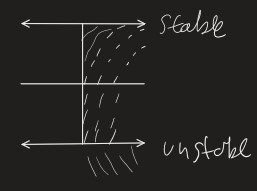
\includegraphics{resource/images/2.7 Example 1.jpg}
    \end{center}

    We need to classify each of the lines here as stable (a sink), unstable (a source), or semi-stable (a node). From this slope diagram we can make a phase diagram.

      

    The arrows in this diagram indiciate wether $\frac{dy}{dx}$ is above or below $0$. We can see that the long term behavior of the solution:

    \begin{equation}
      \begin{aligned}
        y_0 = y(t_0) > 2,\to y(t)\to 2\\
        - 2 < 2_0,\to y(t)\to 2\\
        y_0 <- 2, y(t)\to -\infty\\
      \end{aligned}
    \end{equation}
  \end{problem}

  Let's take a look at another example problem:

  \begin{problem}
    Compare the pivots of the two ordinary differential equations, $\frac{dy}{dt}=y^2(1-y)^2$, and $\frac{dy}{dx}=y^2(1-y^2)$.

    \begin{align}
      \frac{dy}{dt}=y^2(1-y)^2 && \frac{dy}{dt}=y^2(1-y^2)\\
      0=y^2(1-y)^2 && 0=y^2(1-y^2)\\
      && y=0,\pm1\\
    \end{align}
    From finding the equilibrium points of the differential equations, we can now craft a pivot diagram:\newline
    \begin{center}
    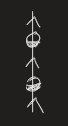
\includegraphics{resource/images/2.7 Example 2-1.jpg}
    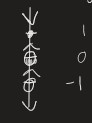
\includegraphics{resource/images/2.7 Example 2-2.jpg}
    \end{center}

    From this we can see that in the long term, the equations are going to look like this:

    \begin{align}
      y_0<0,y(t)\to0\\
      0<y_0<1,y(t)\to1\\
      1<y_0,y(t)\to\infty\\
    \end{align}
  \end{problem}

  \subsection{Biforcations}

  For ordinary differential equations with a parameter, there are times that a small change in the value of the parameter results in a huge change in the behavior of the solutions. It causes a change in the number or stability of the equilibrium solutions.

  \begin{problem}
    Find the biforcation value for 

    \begin{equation}
      \frac{dp}{dt}=0.5p\left(1-\frac{p}{100}\right)-H
    \end{equation}

    The first step for finding a biforcation for an equation is finding the equilibrium solutions. In order to do that, we set equation (2.69) equal to 0 and then rearrange it so it is in the form

    \begin{equation}
      p^2=-100p+250H=0
    \end{equation}

    In this case, we are going to need to use the quadratic formula to find the equilibrium points:

    \begin{align}
      p=\frac{100\pm\sqrt{10000-1000H}}{2}\\
      =50\pm5\sqrt{100-10H}
    \end{align}
    hihihihihi
  \end{problem}